\documentclass{article}
\usepackage[margin=1.0in]{geometry}
\usepackage{amsmath, amssymb, mathrsfs}
\usepackage[english]{babel}
\usepackage{graphicx}
\usepackage{enumerate}
\usepackage{listings}
\usepackage{pgfplots}
\usepackage{tikz}
\renewcommand{\vec}[1]{\mathbf{#1}}

\title{Machine Learning from Data Assignment 2}
\author{Greg Stewart}
\date{\today}

\begin{document}

\maketitle

\subsection*{Exercise 1.8}

\textit{If $\mu = 0.9$, what is the probability that a sample of 10 marbles will have $\nu \leq 0.1$?}


There can be either 0 or 1 red marbles in the 10 marble sample. So we can calculate the
probability of having 0 or any 1 of the marbles be red.

All not red: $0.1^{10} = 10^{-10}$

One red: $10 \cdot (0.1)^{9} \cdot .9 = 9 \times 10^{-9}$

So the overall probability of this event is 

$$9.1 \times 10^{-9}$$


\subsection*{Exercise 1.9}

\begin{align*}
  \mathbb{P}[|\nu - \mu| > \epsilon ] &\leq 2e^{-2\epsilon^2N} \\
  \mathbb{P}[|0.1 - 0.9| > \epsilon ] &\leq 2e^{-20 \epsilon^2} \\
  \intertext{Choosing $\epsilon$ very close to the actual difference, 0.8, we obtain}
  \mathbb{P}[|0.1 - 0.9| > 0.79999 ] &\leq 5.52 \times 10^{-6}
\end{align*}

This is much larger than the probability obtained in the previous exercise, but it is an upper bound, whereas in the previous exercise we computed the actual probability.

\subsection*{Exercise 1.10}

\textit{Experiment: Run a computer simualtion for flipping 1000 fair coins. Flip each coin independently 10 times. Focus on 3 coins as follows: $c_1$ is the first coin flipped; $c_{rand}$ is a coin you choos at random; $c_{min}$ is the coin that had the minimum frequency of heads (picking the earlier one in case of a tie). Let $\nu_1, \nu_{rand}, \nu_{min}$ be the fraction of heads you obtain for the respective three coins.}

\begin{enumerate}[(a)]
  \item \textit{What is $\mu$ for the three coins selected?}

    Since the coins are all fair, $\mu = 0.5$

  \item \textit{Repeat this entire experiment a large number of times to get several instances ofthe $\nu$'s and plot the histograms of the distributions. Notice that which coins end up being $c_{rand}$ and $c{min}$ may differ from one run to another.}

    For this experiment, N = 20,000.
    
    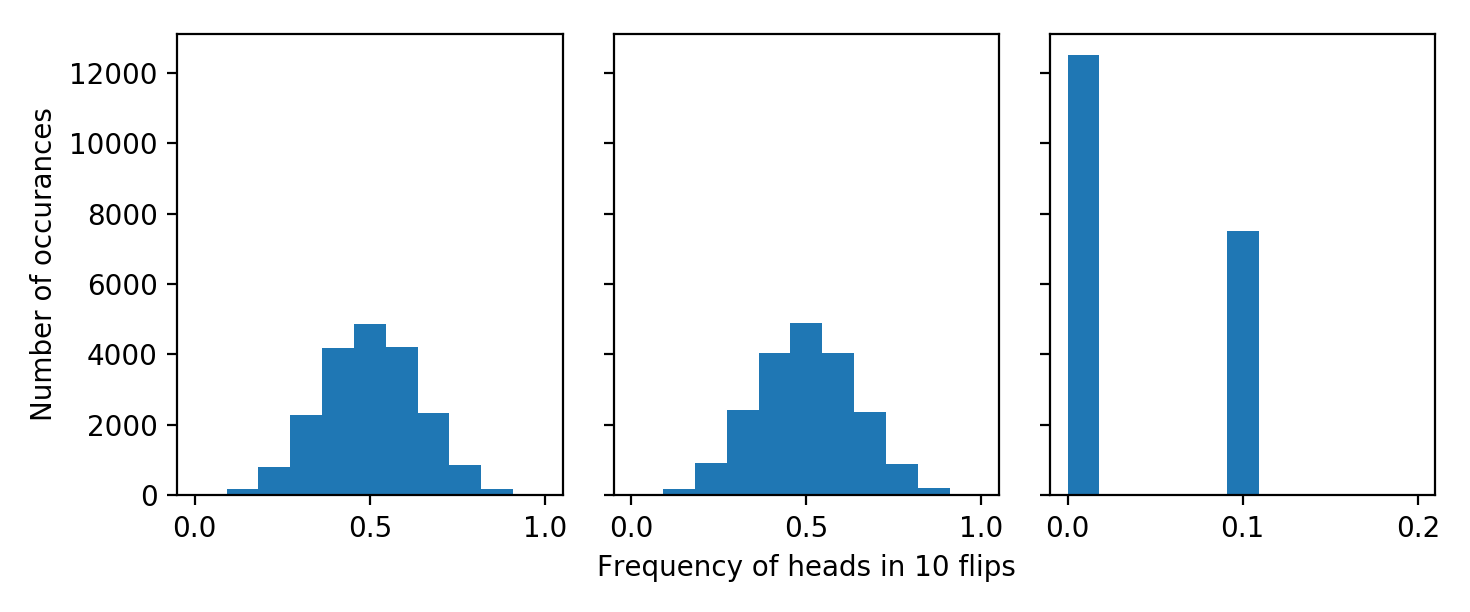
\includegraphics[width=\textwidth]{Figure_1.png}

  \item \textit{Using (b), plot estimates for $\mathbb{P}[|\nu - \mu| > \epsilon]$ as a function of $\epsilon$, together with the Hoeffding bound.}

    \begin{tikzpicture}
    \begin{axis}[
        axis lines = left,
        xlabel = $\epsilon$,
        ylabel = {$f(\epsilon)$},
    ]
    %Below the red parabola is defined
    \addplot [
        domain=0:.0125, 
        samples=300, 
        color=red,
    ]
      {2*e^(-2*20000*x^2)};
    \addlegendentry{Hoeffding Bound}
    %Here the blue parabloa is defined
%   \addplot [
%       domain=-10:10, 
%       samples=100, 
%       color=blue,
%       ]
%       {x^2 + 2*x + 1};
%   \addlegendentry{$x^2 + 2x + 1$}
     
    \end{axis}
    \end{tikzpicture}

  \item \textit{Which coins obey the Hoeffding bound, and which do not?}

    $c_1$ and $c_{rand}$ both obey the Hoeffding bound, while $c_{min}$ does not. This is because $c_{rand}$ is chosen at random each time and is independent of other choices, so as $N$ increases, the mean or expected value of the sample tends to the actual mean. The situation is similar for $c_1$; although choosing $c_1$ each time is a determination made beforehand, the actual outcome is random, and this randomness and independence also applies to the distribution for $c_1$, so we see the same thing. $c_{min}$ does not obey the Hoeffding bound because, due to the random nature of coin-flipping, in a batch of 1000 examples of 10 flips, the minimum frequency of, which just has to occur one time, is likely to be much lower than the mean.

  \item \textit{Relate part (d) to the multiple bins in Fig. 1.10.}

    The distributions for $c_1$ and $c_{rand}$ are obtained in entirely different ways, 
    but give rise to almost the exact same distribution. In both cases, the situation is
    analagou to reaching randomly into a bin to obtain a sample. The $c_{min}$ distribution 
    is obtained in a different way, and provides a completely different sample set which is not 
    distributed like the other two because the sample taken from the "bin" is not obtained
    randomly, but deliberately, taking the minimum.

\end{enumerate}

\subsection*{Exercise 1.11}

\begin{enumerate}[(a)]
  \item \textit{Can S produce a hypothesis that is guaranteed to perform better than random on any point outside D?}


    No, no such guarantee can be made. It can only perform better than random with some probability, not with certainty.


  \item \textit{Assume for the rest of the exercise that all the examples in D have $y_n = +1$. Is it possible that the hypothesis which C produces turns out to be better than the hypothesis that S produces?}

    Yes, it is possible. In this case, S would produce $h_1$ as it matches all of the data. However, it's possible that outside D, the rest of $\mathbb{R}$ maps to $-1$. This would mean C is accurate for the entirety of $\mathbb{R}$, save for the in D, which is literally infinitely better than S.

  \item \textit{If $p = 0.9$, what is the probability that S will produce a better hypothesis than C?}

    We need $$\mathbb{P}[\mathbb{P}[g_S \approx f] > \mathbb{P}[g_C \approx f]]$$

    where $g_S$ is the resulting hypothesis from S and $g_C$ the result from C.

    Since $\mathbb{P}[f(x) = +1] = 0.9$, we can say $\mathbb{P}[g_s \approx f] = 0.9$.
    The analagous probability for $g_C$ is 0.5, for both the +1 and -1 cases. We can now
    calculate the probability $$\mathbb{P}[g_C \approx f] = 0.5(0.9) + 0.5(0.1) = 0.5$$.

    We know that $\mathbb{P}[g_S \approx f] = 0.9$, and $0.9 > 0.5$, so 

    $$\mathbb{P}[\mathbb{P}[g_S \approx f] > \mathbb{P}[g_C \approx f]] = 1$$


  \item \textit{Is there any value for $p$ for which it is more likely than no that C will produce a better hypothesis than S?}

    Yes---for $p < 0.5$ this will be the case.


\end{enumerate}


\subsection*{Exercise 1.12}

The answer is (c). If learning succeeds, and a hypothesis $g$ is produced, then we can be reasonably sure, to a high probability, that $g \approx f$. But there is the chance the learning will fail, in which case the only thing to do is declare the failure.





\end{document}
